\documentclass[journal]{IEEEtran}
\usepackage{cite}
\usepackage{amsmath,amssymb}
\usepackage{graphicx}
\usepackage{textcomp}
\usepackage{booktabs}
\usepackage{url}
\usepackage{placeins}

\graphicspath{{figures/}}

\begin{document}


\title{An Activity-Rate-Aware Hysteresis Controller for Lightweight Adaptive Power Gating in SoC Functional Blocks}

\author{
\IEEEauthorblockA{
\textbf{Authors:} Joud Thaher \& Layan Salem\\
\textbf{Supervisor:} Dr.\ Khader Mohammed\\
\textbf{Department:} Electrical and Computer Engineering\\
\textbf{University:} Birzeit University, Palestine\\
\textbf{GitHub Repository:} \url{https://github.com/JHT127/hysteresis-adaptive-power-gating}
}
}

\maketitle


\begin{abstract}
Conventional power-gating controllers for small SoC functional blocks typically select sleep states using idle-cycle count alone, a policy that is vulnerable to thrashing -- repeated, costly sleep/wake transitions -- under bursty workloads. This work proposes a lightweight power-gating controller for a 32-bit ALU block that gates sleep-state entry on the conjunction of consecutive idle-cycle count and a rolling-window activity rate, with adaptive widening of entry thresholds during high-activity periods. The controller is implemented in synthesizable RTL with three power states (ON, Light Sleep, Deep Sleep) and is evaluated against a fixed-threshold baseline representative of prior multi-level power-gating work, using an identical ALU, isolation strategy, and UPF power intent for both designs. Functional simulation across burst, sparse, and mixed workloads shows the proposed controller eliminates thrashing under bursty traffic (zero mode transitions vs.\ nineteen for the baseline, preserving throughput at 59.3\% vs.\ 19.3\%), while converging to comparable leakage savings under unambiguous idle conditions (31.6\% vs.\ 33.4\%). Synthesis at two clock corners (5\,ns and 2\,ns) and full place-and-route in a 14\,nm standard-cell library using Synopsys Fusion Compiler show a real post-route area overhead of 13.6\% with identical, fully met timing closure on both designs and zero open nets after routing. Results indicate that the proposed dual-condition policy trades a bounded, modest area cost for a substantial improvement in throughput stability under realistic bursty traffic -- a trade-off not previously quantified for comparator-based (non-machine-learning) adaptive power-gating controllers at this scale.
\end{abstract}

\begin{IEEEkeywords}
power gating, adaptive power management, leakage power, low-power VLSI, hysteresis control, multi-level sleep, RTL design, ASIC implementation, SAED 14nm
\end{IEEEkeywords}

\section{Introduction}

Leakage power has become a dominant component of total power dissipation as CMOS technology scales into deep-submicron and nanometer nodes, particularly for blocks that spend significant fractions of their operating lifetime idle \cite{shiva2025,sahu2025}. Power gating -- disconnecting idle logic from its supply rail via sleep transistors -- remains one of the most widely deployed leakage-reduction techniques in commercial SoC design, but the \emph{policy} governing when to gate is frequently static: a fixed number of idle cycles triggers sleep entry, regardless of how that idle period arose \cite{agarwal2006}.

This static-threshold approach has a known failure mode. A workload composed of short, frequent bursts separated by gaps that individually exceed the sleep-entry threshold will cause the controller to repeatedly enter and exit sleep states -- thrashing -- even though the block is, in aggregate, far from idle. Each entry/exit cycle incurs a wake-up latency penalty and, in deep-submicron designs, a rush-current and ground-bounce cost during reactivation \cite{chang2012}. The leakage saved by sleeping briefly can be outweighed by the throughput and energy cost of waking up repeatedly.

Recent work has approached this problem from two directions. Multi-level sleep-mode controllers \cite{agarwal2006} introduce intermediate power states with different leakage/wake-up-latency trade-offs, but still gate transitions on idle-cycle count alone. Workload-adaptive controllers using machine-learning techniques -- clustering and recurrent prediction -- have been proposed for multi-core systems \cite{karthikeyan2025}, achieving strong adaptivity at the cost of prediction-hardware overhead that is difficult to justify for a single small functional block.

This work proposes a middle path: a comparator-based (non-machine-learning) hysteresis controller that gates sleep-state entry on the \emph{conjunction} of idle-cycle count and a rolling-window activity rate, widening its entry thresholds when recent activity indicates a bursty rather than genuinely idle workload. This work makes the following contributions:

\begin{itemize}
\item A dual-condition sleep-entry policy combining idle-cycle count and activity rate, implemented with a 16-cycle shift-register popcount and simple comparators -- no multipliers, no learned models.
\item Adaptive threshold widening that suppresses sleep entry during bursty operation without per-cycle software classification.
\item A fair, single-module-substitution comparison methodology against a fixed-threshold baseline sharing identical ALU, isolation, retention, and UPF infrastructure, isolating the decision-logic contribution as the sole experimental variable.
\item A quantitative characterization, at both RTL-simulation and post-route physical-implementation levels, of the throughput-stability/area trade-off this policy introduces.
\end{itemize}

The remainder of this paper is organized as follows. Section~\ref{sec:related} reviews related power-gating and adaptive power-management work. Section~\ref{sec:architecture} describes the proposed architecture. Section~\ref{sec:methodology} details the implementation and experimental methodology. Section~\ref{sec:results} presents results. Section~\ref{sec:discussion} discusses findings and limitations. Section~\ref{sec:conclusion} concludes.
\section{Background and Related Work}
\label{sec:related}

Agarwal et al. \cite{agarwal2006} established the multi-level sleep-mode concept this work builds on, defining sleep depths with different footer gate-bias levels and demonstrating that allowing an intermediate, state-retentive mode in addition to full cutoff yields a further 17\% leakage reduction over single-mode gating, with the retentive mode itself saving 19\% leakage while preserving circuit state. Their decision policy, however, selects mode purely from idle-cycle count against fixed thresholds; the present work adopts their mode-hierarchy concept directly but replaces the decision logic.

Chang et al. \cite{chang2012} address a complementary problem: once a sleep-mode transition has been decided, how to execute the wake-up safely. Their two-phase footer activation -- enabling a small transistor fraction before the full width -- reduces wake-up time by approximately 10\% while bounding power-supply bounce. This work's sleep controller adopts the same two-phase activation principle for both the baseline and proposed designs, so it is held constant across the comparison reported here; the contribution of this work is orthogonal, addressing the entry-decision policy rather than the transition mechanism.

Karthikeyan et al. \cite{karthikeyan2025} propose workload-adaptive power management for multi-core systems combining real-time monitoring, dynamic voltage and frequency scaling, and core-level gating, using K-means clustering and recurrent neural prediction to classify workload intensity. Reported savings of up to 35\% and meaningful thermal reduction demonstrate the value of activity-aware adaptation, but the prediction hardware is sized for multi-core systems and is difficult to justify for a single small block such as the one considered here. This work targets the same underlying goal -- workload-character-aware adaptation -- using a fixed-function comparator network rather than a learned model.

Surveys by Shiva and Patil \cite{shiva2025} and Sahu et al. \cite{sahu2025} situate power gating within the broader landscape of low-power VLSI techniques (dynamic voltage scaling, clock gating, multi-threshold CMOS), both noting that AI-assisted predictive management is an emerging direction but that lightweight, non-learned alternatives remain comparatively underexplored for fine-grained blocks. Tong et al. \cite{tong2024} address adaptive energy management in an unrelated domain (mobile edge computing task offloading), offering a Lyapunov-based stability framework for resource allocation under stochastic load; while not directly applicable to gate-level power gating, the queue-stability framing motivates this work's attention to throughput preservation, not leakage savings alone, as an evaluation criterion.

Table~\ref{tab:related} summarizes the approach, key strength, and remaining gap of each reviewed work relative to the present contribution.

%% ── Table: Related work comparison ───────────────────────────────────────
\begin{table*}[t]
\centering
\footnotesize
\caption{Comparison of Related Work in Power Gating and Adaptive Power Management}
\label{tab:related}
\setlength{\tabcolsep}{3pt}
\renewcommand{\arraystretch}{1.3}
\begin{tabular}{@{}p{2.3cm} p{3.3cm} p{3.6cm} p{3.6cm} p{3.9cm}@{}}
\toprule
\textbf{Reference} & \textbf{Approach} & \textbf{Key Strength} & \textbf{Key Limitation} & \textbf{Gap Addressed by This Work} \\
\midrule
Agarwal et al.\ \cite{agarwal2006} &
MTCMOS multi-level power gating (Active/Light Sleep/Deep Sleep) with fixed idle-cycle thresholds &
Proven leakage savings; retentive intermediate mode cuts leakage by a further 17\% &
Static thresholds; no activity-rate check, prone to thrashing under bursty idle gaps &
Adopts the mode hierarchy directly but replaces the fixed-threshold decision logic with a dual-condition, activity-rate-aware gate \\
\addlinespace
Chang et al.\ \cite{chang2012} &
Two-phase footer activation for rush-current-controlled wake-up &
Reduces wake-up time by $\sim$10\% while bounding supply bounce &
Addresses only the wake-up transition mechanism; no sleep-entry decision logic &
Adopts the wake-up mechanism unchanged in both baseline and proposed designs; contribution is orthogonal (entry policy, not transition) \\
\addlinespace
Karthikeyan et al.\ \cite{karthikeyan2025} &
ML-based workload monitoring, DVFS, and core-level power gating for multi-core SoCs &
Full-stack adaptive power management; reported savings up to 35\% &
Clustering/recurrent-prediction hardware overhead is difficult to justify for a single small block &
Achieves comparable qualitative adaptivity with a fixed-function comparator network -- no learned model, no inference hardware \\
\addlinespace
Shiva and Patil \cite{shiva2025} &
Survey of DVS, power gating, and clock-gating optimization techniques &
Comprehensive overview of the low-power VLSI landscape &
No new architecture or hardware implementation proposed &
Identifies lightweight, non-learned adaptive gating as underexplored, motivating this work's scope \\
\addlinespace
Sahu et al.\ \cite{sahu2025} &
Design-optimization survey for low-power VLSI circuits in high-performance computing &
Broad, practically grounded design-optimization perspective &
No adaptive, rate-aware sleep-entry logic proposed &
Reinforces the same gap; this work supplies a concrete circuit-level instantiation \\
\addlinespace
Tong et al.\ \cite{tong2024} &
Lyapunov-based stability framework for resource allocation in IIoT task offloading &
Principled queue-stability framing for throughput-aware adaptation &
Different domain (network resource allocation); not applicable at gate level &
Motivates evaluating throughput preservation, not leakage savings alone, as a first-class metric \\
\bottomrule
\end{tabular}
\end{table*}

No reviewed work combines a non-learned, comparator-based dual-condition (idle-count and activity-rate) sleep-entry policy with adaptive threshold widening, evaluated against a fair, structurally matched fixed-threshold baseline at both RTL-simulation and post-route physical-implementation levels. This is the contribution of the present work.
\section{Proposed Architecture}
\label{sec:architecture}

\begin{figure}[t]
\centering
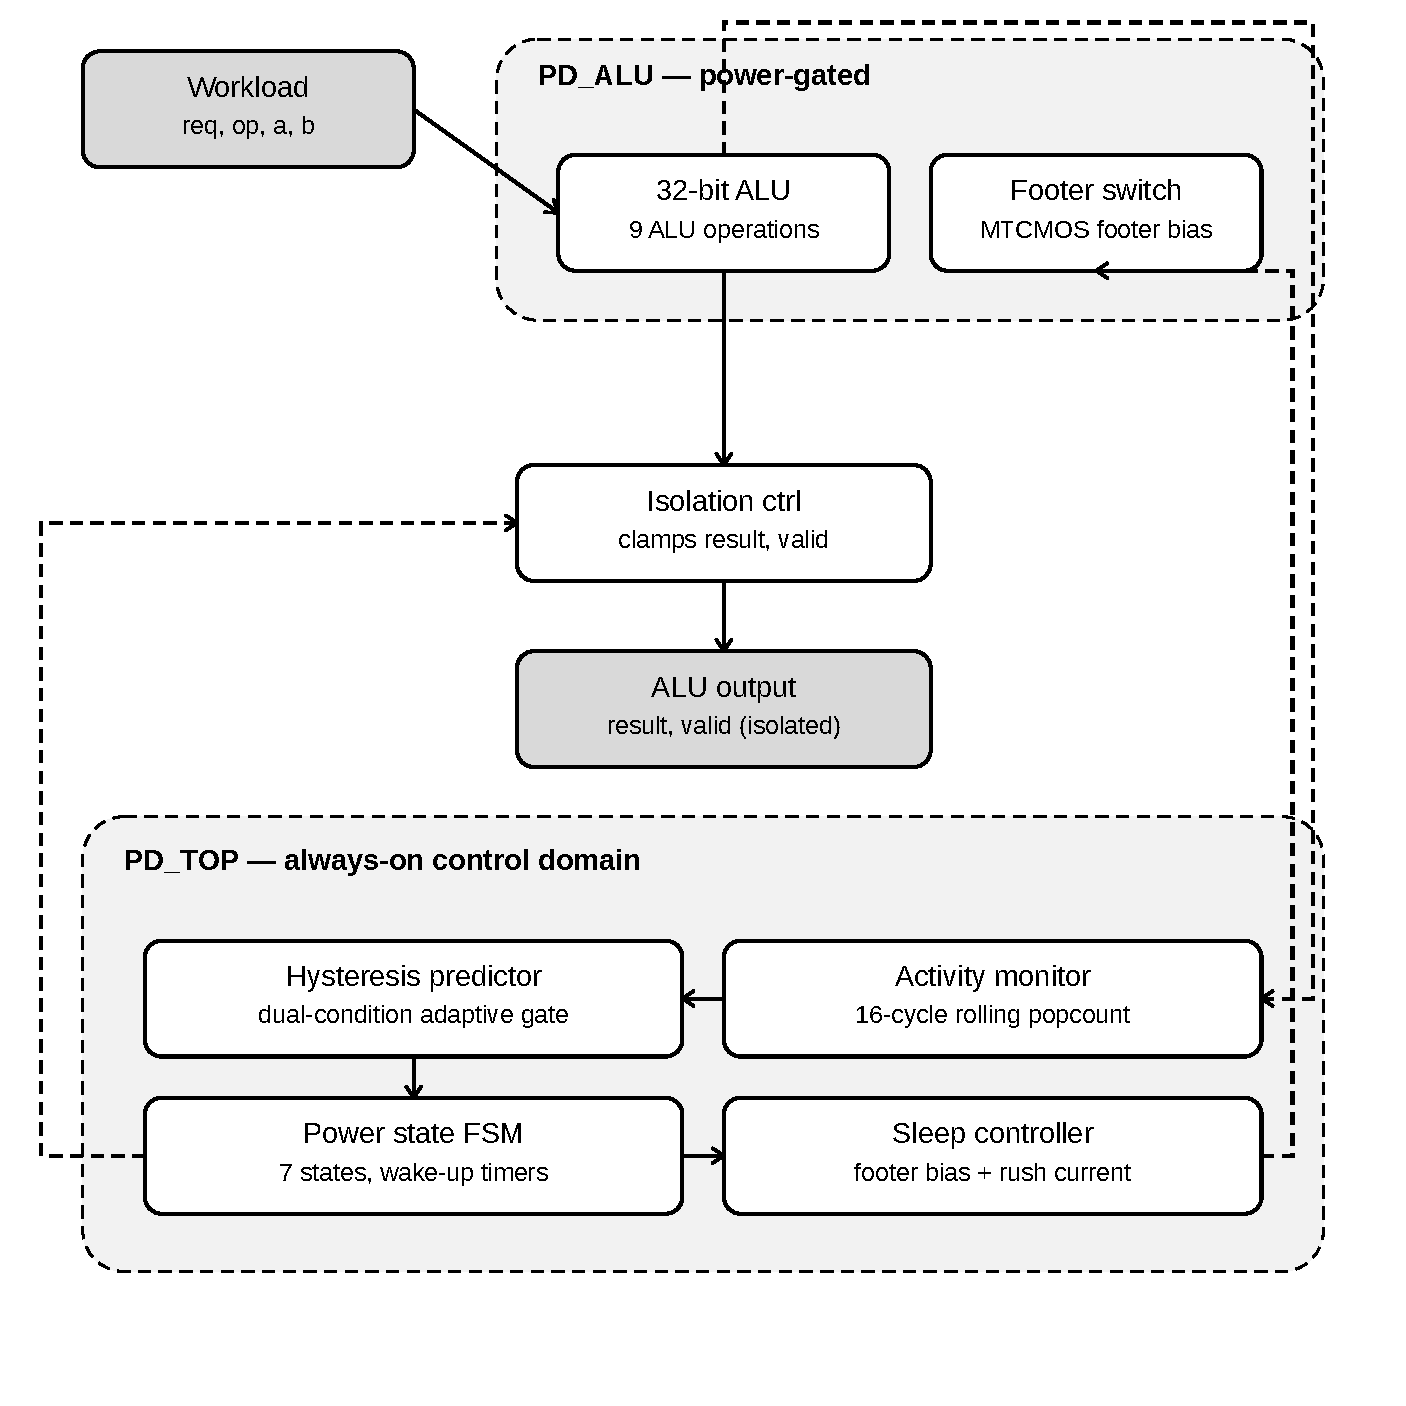
\includegraphics[width=\columnwidth]{fig1_architecture.pdf}
\caption{Architecture of the adaptive multi-level power-gating controller, showing the two UPF power domains (\textsf{PD\_ALU}, power-gated; \textsf{PD\_TOP}, always-on) and inter-module signal flow.}
\label{fig:architecture}
\end{figure}

The controller is organized into two power domains (Fig.~\ref{fig:architecture}), following the UPF power-intent model. \textsf{PD\_TOP}, the always-on domain, contains the activity monitor, hysteresis predictor, power-state finite state machine (FSM), and sleep controller. \textsf{PD\_ALU}, the power-gated domain, contains the 32-bit ALU functional block and its MTCMOS footer switch. Fig.~\ref{fig:baseline_vs_proposed} shows both the baseline and proposed top-level architectures side by side, highlighting the single substituted module.

\begin{figure}[t]
\centering
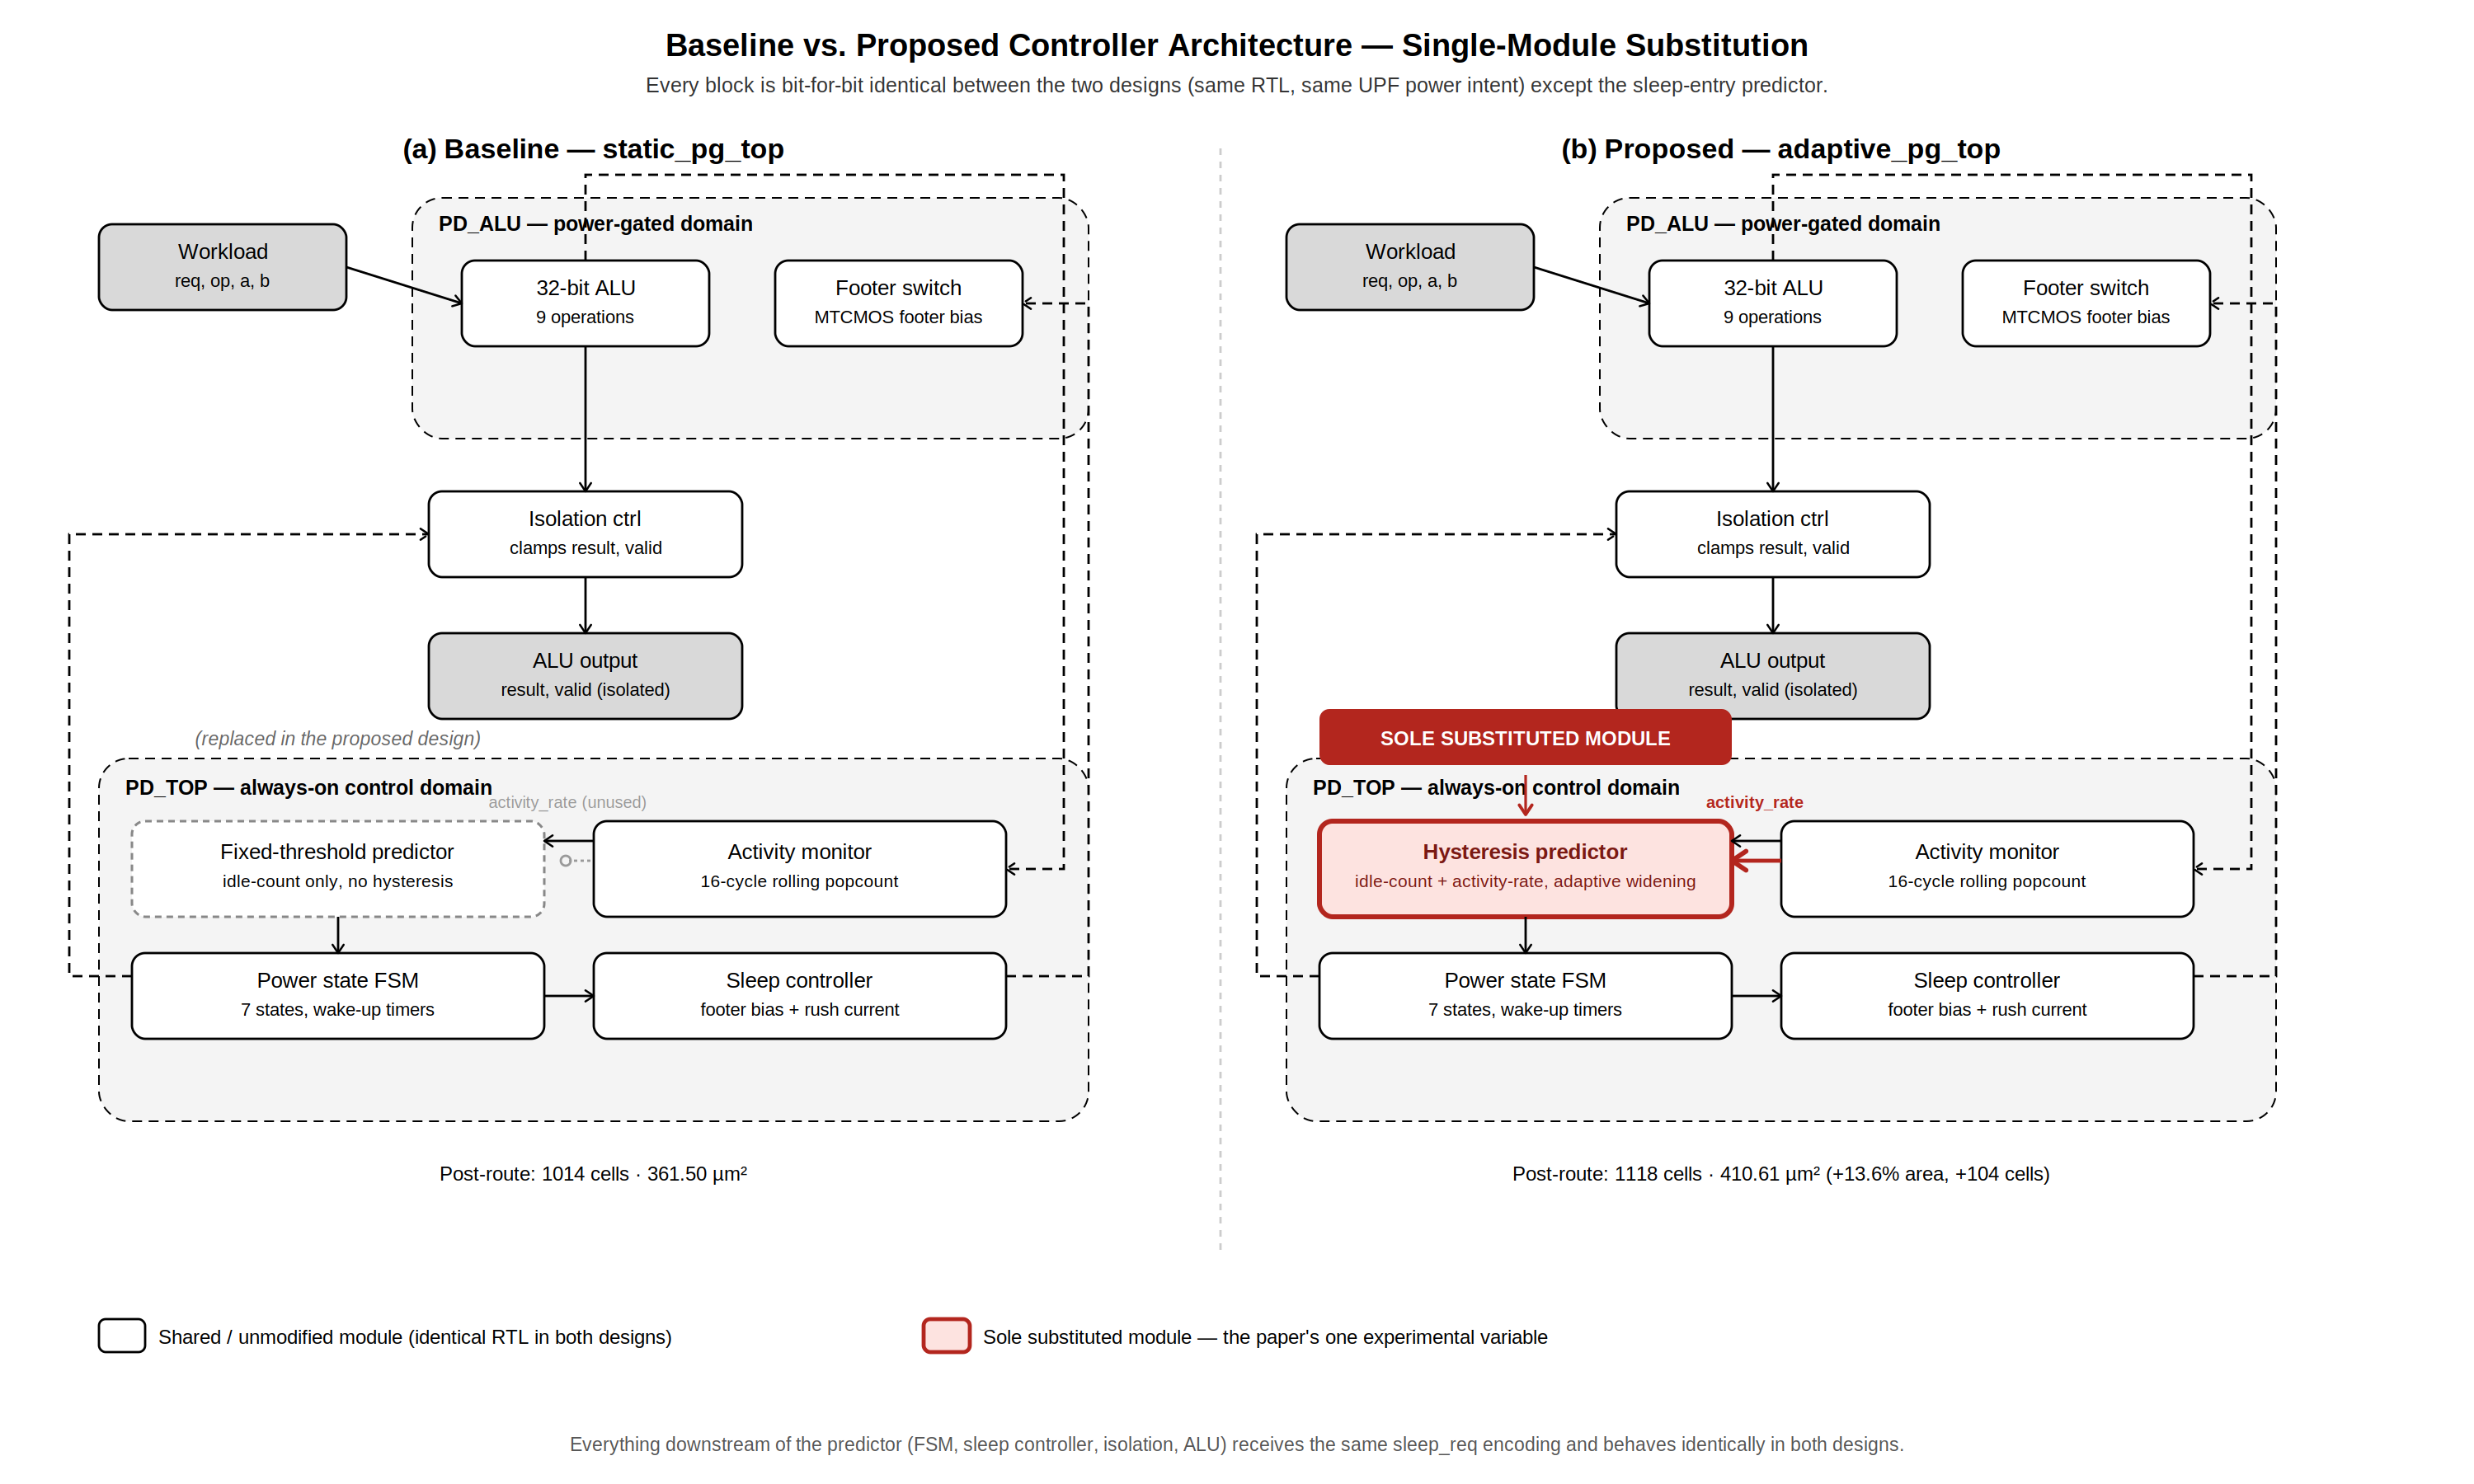
\includegraphics[width=\columnwidth]{fig1b_baseline_vs_proposed.png}
\caption{Baseline vs.\ proposed controller architecture under the single-module substitution protocol. Every block is bit-for-bit identical between the two designs except the sleep-entry predictor (highlighted in red). Post-route instance counts and area are shown for reference.}
\label{fig:baseline_vs_proposed}
\end{figure}

\subsection{Activity Monitor}
The activity monitor implements a 16-cycle rolling window as a shift register, computing a consecutive-idle-cycle count and an activity rate (fraction of the window with observed activity, scaled to an 8-bit range) using only shift and population-count logic -- no multipliers. Every cycle, a 1 is shifted in if the ALU was active, or a 0 if idle. The population count of the window gives the activity rate.

\subsection{Hysteresis Predictor}
The hysteresis predictor is the controller's central novel contribution. It requests a sleep-state transition only when \emph{both} the idle-cycle count exceeds a mode-specific threshold \emph{and} the activity rate is below a corresponding ceiling; further, when the activity rate exceeds a configurable high-activity threshold (\texttt{HIGH\_RATE\_THRESH}~$= 192/255$), both entry thresholds are widened by a fixed offset (\texttt{ADAPT\_OFFSET}~$= 6$~cycles), suppressing sleep entry during workloads that are bursty rather than genuinely idle. Separate, narrower exit thresholds create hysteresis bands that prevent rapid oscillation between states.

The dual-condition sleep-entry gate operates as follows:
\begin{align}
\text{enter\_LS} &= (\texttt{idle\_count} > \theta_\text{LS}) \wedge (\texttt{rate} < R_\text{LS}) \label{eq:ls}\\
\text{enter\_DS} &= (\texttt{idle\_count} > \theta_\text{DS}) \wedge (\texttt{rate} < R_\text{DS}) \label{eq:ds}
\end{align}
where $\theta_\text{LS}$ and $\theta_\text{DS}$ are the adaptive thresholds:
\begin{equation}
\theta_i = \begin{cases} \theta_{i,\text{base}} + \Delta & \text{if } \texttt{rate} > T_\text{high} \\ \theta_{i,\text{base}} & \text{otherwise} \end{cases}
\label{eq:adaptive}
\end{equation}
with $\theta_\text{LS,base}=4$, $\theta_\text{DS,base}=8$, $\Delta=6$, $R_\text{LS}=80$, $R_\text{DS}=32$, and $T_\text{high}=192$ (all in 8-bit counts or fractions of 255).

Figs.~\ref{fig:baseline_gatelevel} and~\ref{fig:proposed_gatelevel} show the synthesized gate-level schematics of the baseline and proposed predictors respectively, extracted from the DC Ultra netlist. The baseline predictor (Fig.~\ref{fig:baseline_gatelevel}) uses only \texttt{idle\_count[7:0]} as input, implementing threshold comparison through an OR4NR2INVAO32 chain with two output flip-flops (FDP, FSDPQB) -- a total of approximately 6~standard cells. The proposed predictor (Fig.~\ref{fig:proposed_gatelevel}) adds \texttt{activity\_rate[7:0]} as a second input port, requiring additional NR2, AOI21, OAI21, and OR4 cells to implement the conjunction of both conditions and the hysteresis state -- approximately 16~standard cells. The 104-cell post-route overhead between the two designs includes this predictor difference plus the additional comparator and MUX logic implementing the adaptive threshold widening (Eq.~\ref{eq:adaptive}).

\begin{figure}[t]
\centering
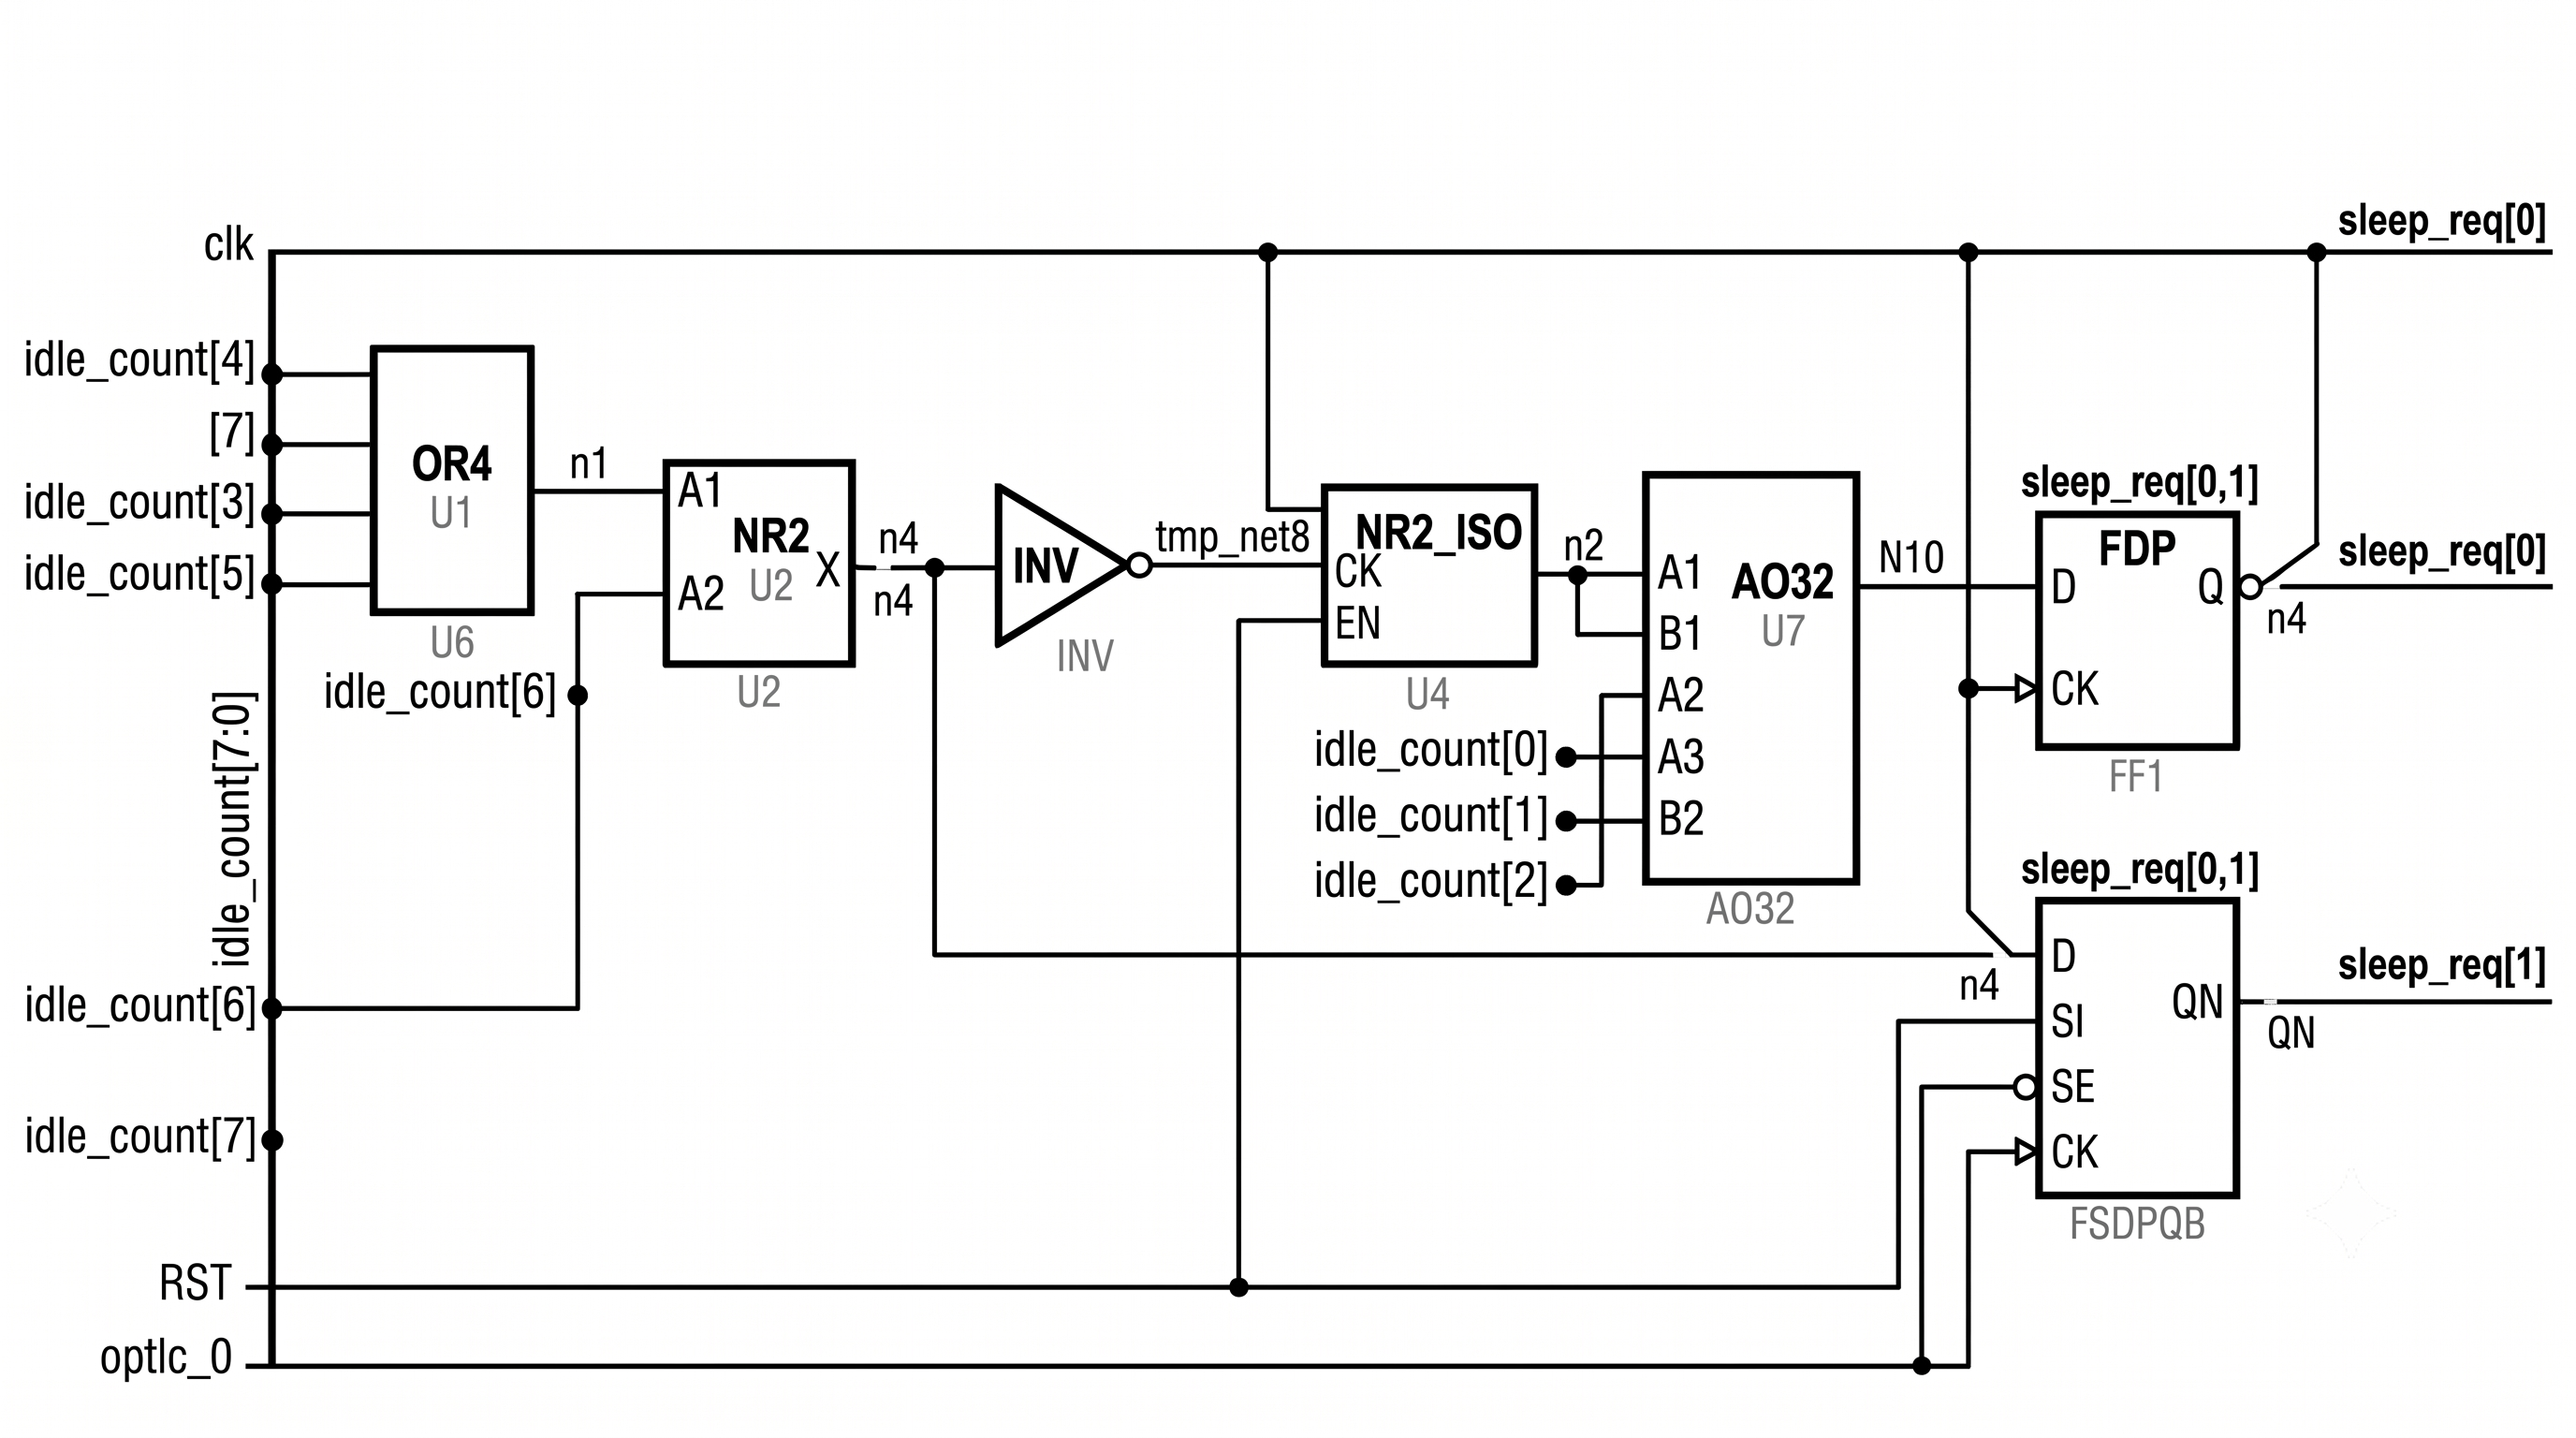
\includegraphics[width=\columnwidth]{fig8_baseline_gatelevel.png}
\caption{Synthesized gate-level schematic of the \emph{baseline} fixed-threshold predictor (DC Ultra, SAED 14\,nm LVT). Only \texttt{idle\_count[7:0]} is consumed; \texttt{activity\_rate} is not connected. The decision logic reduces to a single OR4NR2INVAO32 comparator chain followed by two output registers ($\approx$6 standard cells).}
\label{fig:baseline_gatelevel}
\end{figure}

\begin{figure}[t]
\centering
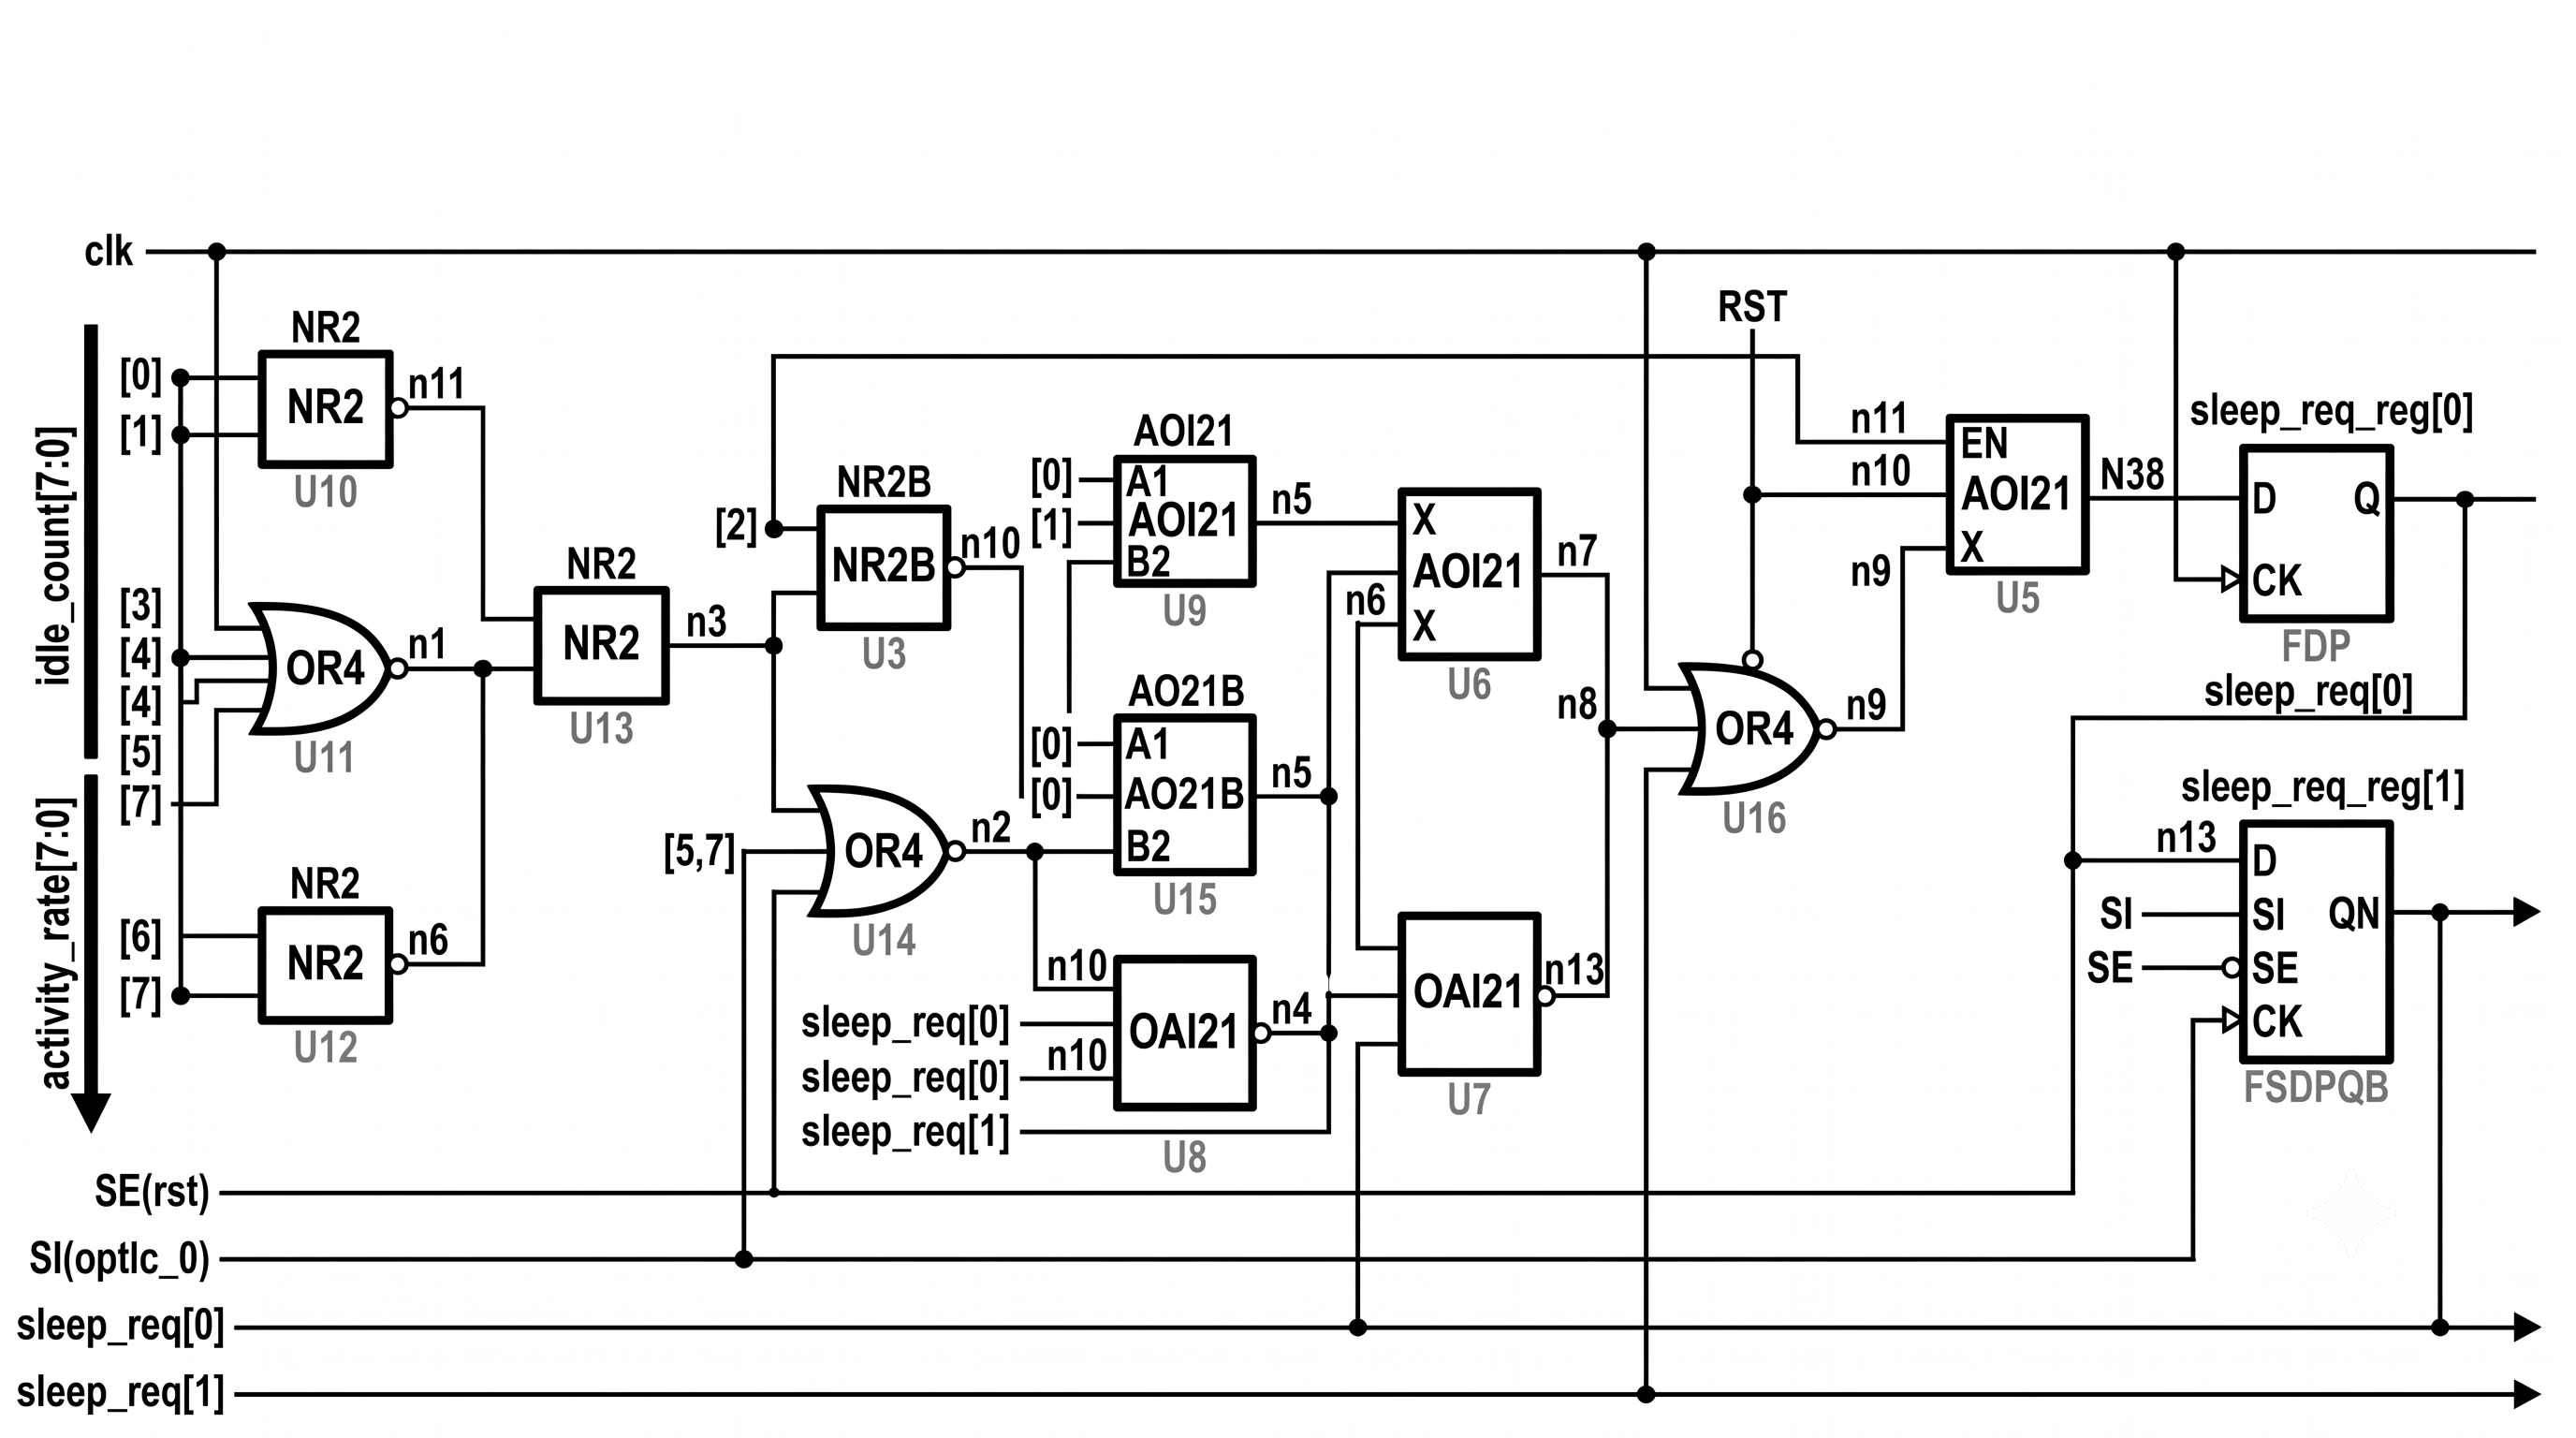
\includegraphics[width=\columnwidth]{fig9_proposed_gatelevel.png}
\caption{Synthesized gate-level schematic of the \emph{proposed} hysteresis predictor (DC Ultra, SAED 14\,nm LVT). Both \texttt{idle\_count[7:0]} and \texttt{activity\_rate[7:0]} are consumed. The additional NR2, AOI21, OAI21, and OR4 cells implement the dual-condition AND gate and hysteresis state logic ($\approx$16 standard cells), with output registered in FDP and FSDPQB flip-flops.}
\label{fig:proposed_gatelevel}
\end{figure}

\begin{figure}[t]
\centering
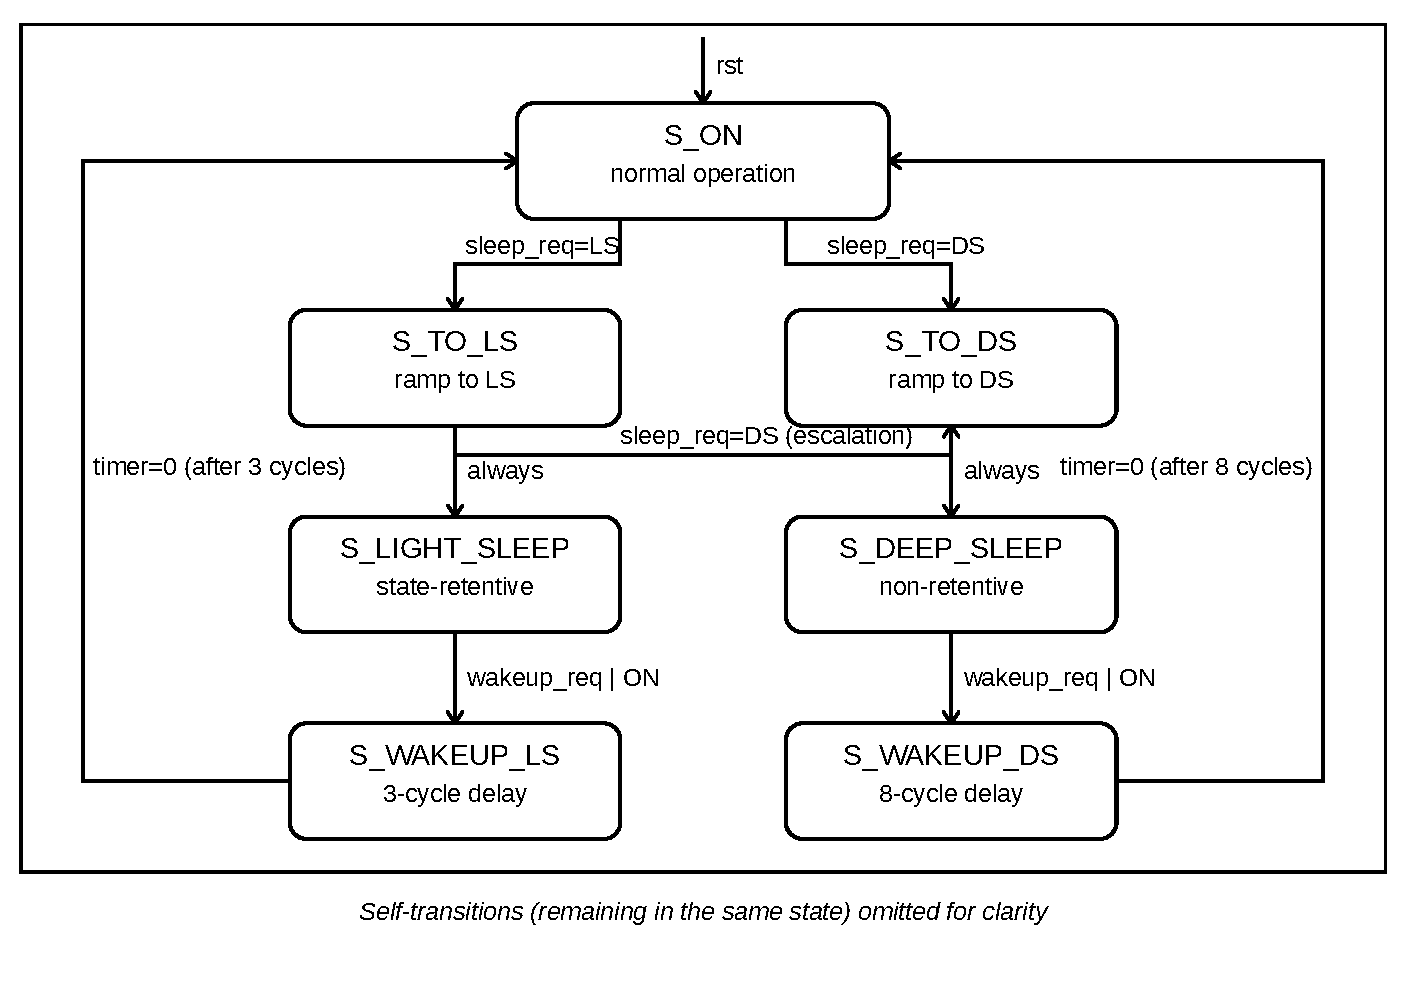
\includegraphics[width=\columnwidth]{fig2_fsm.pdf}
\caption{Power-state FSM, showing all seven states and the conditions governing transitions between them. Self-transitions are omitted for clarity.}
\label{fig:fsm}
\end{figure}

\subsection{Power-State FSM}
The power-state FSM (Fig.~\ref{fig:fsm}) mediates between the predictor's requested mode and the physically realized power state, inserting fixed wake-up-latency delays (3~cycles from Light Sleep, 8~cycles from Deep Sleep) and asserting isolation one cycle before the sleep signal to the power domain, ensuring no floating or undefined values propagate from the gated domain during a transition. The FSM has seven states: \texttt{S\_ON}, \texttt{S\_TO\_LS}, \texttt{S\_LIGHT\_SLEEP}, \texttt{S\_TO\_DS}, \texttt{S\_DEEP\_SLEEP}, \texttt{S\_WAKEUP\_LS}, and \texttt{S\_WAKEUP\_DS}. Leakage in Light Sleep is approximately 81\% of ON-state leakage; Deep Sleep reduces leakage to approximately 64\% of ON-state leakage.

\subsection{Sleep Controller and Isolation}
The sleep controller sequences the footer transistor's gate bias across four levels (active, two intermediate biases, full cutoff) and implements two-phase rush-current control during wake-up, following \cite{chang2012}. The isolation controller clamps the ALU's output and valid signal to a safe constant whenever the domain is not fully powered, modeled as the behavioral equivalent of standard-cell ISO\_AND isolation cells inserted automatically by the physical-design tool under UPF control.

\section{Implementation and Methodology}
\label{sec:methodology}

\subsection{Baseline Design}
To isolate the hysteresis predictor's contribution as the sole experimental variable, a baseline controller was constructed via single-module substitution: the hysteresis predictor is replaced with a fixed-threshold predictor implementing Agarwal et al.'s idle-cycle-count-only policy \cite{agarwal2006} -- no activity-rate input, no hysteresis band (entry and exit thresholds equal), no adaptive widening. Every other module -- the ALU, activity monitor, power-state FSM, sleep controller, isolation controller, and UPF power intent -- is shared, unmodified, between baseline and proposed designs (Fig.~\ref{fig:baseline_vs_proposed}). Threshold values are matched: $\theta_\text{LS,base}=3$ and $\theta_\text{DS,base}=8$ for the baseline predictor, equal to the proposed design's base thresholds before any widening.

\subsection{RTL and Verification}
Both designs are implemented in synthesizable Verilog and verified in Synopsys VCS (T-2022.06-SP2) against a shared, parameterized testbench applying identical stimulus to both designs under burst, sparse, and mixed workload patterns. A correctness checker confirms zero output mismatches between designs whenever both report valid results, confirming the substitution introduces no functional regression in the shared datapath. VCD waveform files were generated for validation; Fig.~\ref{fig:waveform} shows a representative waveform excerpt from the SPARSE workload.

\begin{figure}[t]
\centering
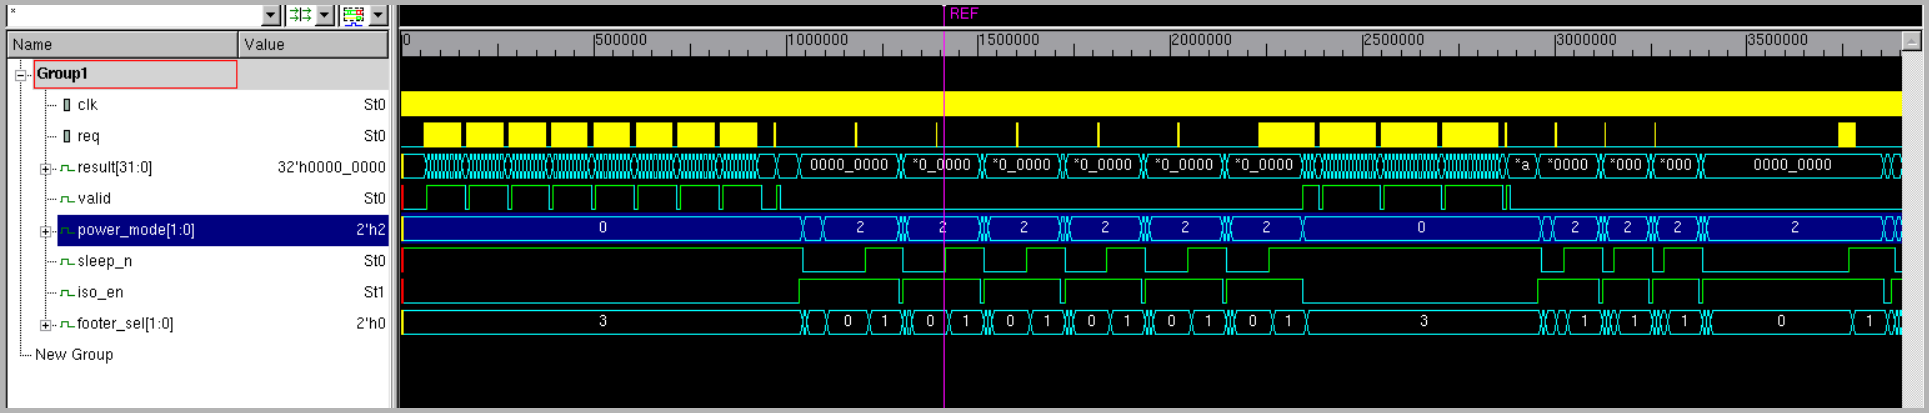
\includegraphics[width=\columnwidth]{fig7_waveform.png}
\caption{VCS simulation waveform (SPARSE workload, time 1.41.9\,ms). The controller enters Deep Sleep (\texttt{power\_mode}=2, \texttt{sleep\_n}=0, \texttt{iso\_en}=1) during long idle periods and executes the 8-cycle wake-up sequence (\texttt{power\_mode}: 2$\rightarrow$0$\rightarrow$1) when \texttt{req} is asserted. Isolation deasserts exactly one cycle after \texttt{sleep\_n} rises, confirming correct sequencing.}
\label{fig:waveform}
\end{figure}

\subsection{Synthesis and Physical Implementation}
Both designs were synthesized in Synopsys Design Compiler Ultra (R-2020.09-SP5) against a 14\,nm low-voltage-threshold standard-cell library (SAED14LVT, \texttt{saed14lvt\_tt0p8v25c}) at two clock corners: low-power (LP) at 5\,ns (200\,MHz) and high-speed (HS) at 2\,ns (500\,MHz), with clock-gating insertion enabled and leakage optimization active. Both designs were subsequently placed, clock-tree-synthesized, and routed in Synopsys Fusion Compiler (U-2022.12-SP5) at the 5\,ns corner. The floorplan was initialized at 30$\times$30\,$\mu$m$^2$ with 2\,$\mu$m core offset, achieving 45.83\% core utilization. Power and ground connections were established for 2,287 pins. Placement completed with zero violations; routing completed with zero open nets and 9,873\,$\mu$m total wire length. Post-route worst negative slack is 3.25\,ns (MET). The post-route layout is shown in Fig.~\ref{fig:layout}.

\begin{figure}[t]
\centering
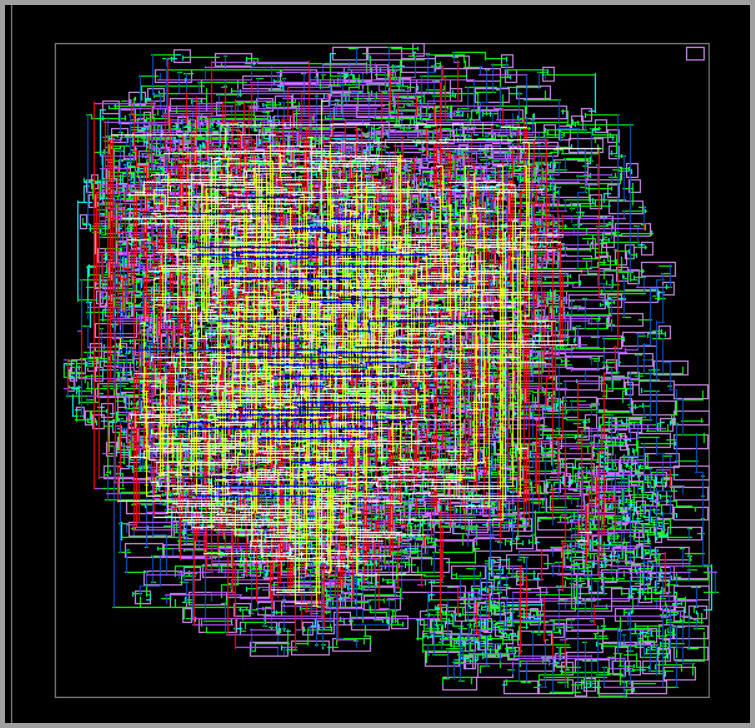
\includegraphics[width=\columnwidth]{fig5_layout_full.png}
\caption{Post-route layout of the proposed \texttt{adaptive\_pg\_top} design in SAED 14\,nm LVT (Synopsys Fusion Compiler U-2022.12-SP5). Die area: 30$\times$30\,$\mu$m$^2$, core utilization: 45.83\%, 1,118 standard-cell instances, 9,873\,$\mu$m total wire length, 0 open nets. Metal routing layers M1M9 are visible.}
\label{fig:layout}
\end{figure}

\begin{figure}[t]
\centering
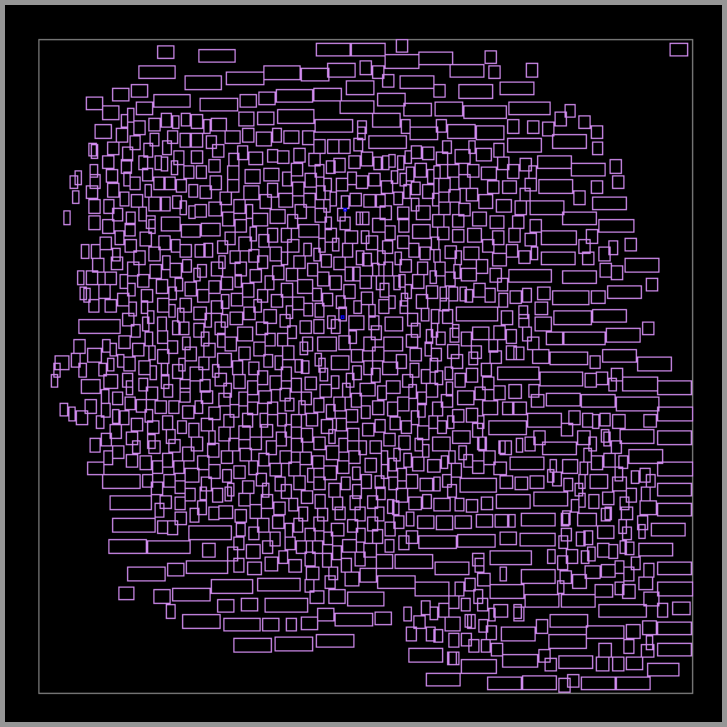
\includegraphics[width=\columnwidth]{fig6_layout_placement.png}
\caption{Cell placement view with all routing layers hidden, showing the 1,118 SAED 14\,nm LVT standard-cell instances distributed across the 30$\times$30\,$\mu$m$^2$ core area at 45.83\% utilization.}
\label{fig:placement}
\end{figure}

\subsection{Experimental Design}
Three synthetic workloads -- burst (frequent short bursts with idle gaps exceeding the baseline's fixed threshold but maintaining duty cycle above the proposed design's activity-rate widening trigger), sparse (long, unambiguous idle periods), and mixed (alternating dense and sparse phases) -- were applied to both designs with identical pseudo-random operand stimulus, with per-mode cycle counts, transition counts, wake-up events, and valid-result throughput logged for each.

\section{Results}
\label{sec:results}

\subsection{Functional Comparison}

\begin{figure*}[t]
\centering
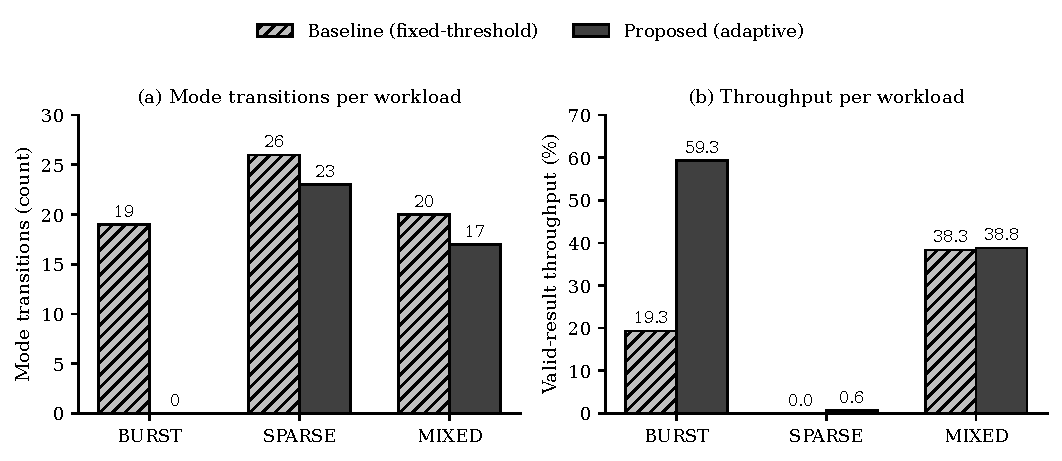
\includegraphics[width=\textwidth]{fig3_functional_comparison.pdf}
\caption{(a) Mode transitions and (b) valid-result throughput, baseline vs.\ proposed, across the three evaluated workloads.}
\label{fig:functional}
\end{figure*}

Table~\ref{tab:cycles} reports per-mode cycle distribution across the three workloads; Table~\ref{tab:functional} reports transition counts, throughput, and leakage savings; Fig.~\ref{fig:functional} visualizes the key results.

%% ── Table I: Cycle distribution ──────────────────────────────────────────
\begin{table*}[t]
\centering
\small
\caption{Per-Mode Cycle Distribution Across Workloads (Baseline vs.\ Proposed)}
\label{tab:cycles}
\setlength{\tabcolsep}{6pt}
\begin{tabular}{l rr rr rr}
\toprule
 & \multicolumn{2}{c}{\textbf{BURST}} & \multicolumn{2}{c}{\textbf{SPARSE}} & \multicolumn{2}{c}{\textbf{MIXED}} \\
\cmidrule(lr){2-3}\cmidrule(lr){4-5}\cmidrule(lr){6-7}
Power State & Base. & Prop. & Base. & Prop. & Base. & Prop. \\
\midrule
Cycles ON              & 78  & 135 & 8   & 16  & 92  & 104 \\
Cycles Light Sleep     & 57  & 0   & 10  & 11  & 10  & 9   \\
Cycles Deep Sleep      & 0   & 0   & 155 & 146 & 81  & 70  \\
Total cycles           & 135 & 135 & 173 & 173 & 183 & 183 \\
\bottomrule
\end{tabular}
\end{table*}

%% ── Table II: Functional metrics ─────────────────────────────────────────
\begin{table*}[t]
\centering
\small
\caption{Functional Performance Metrics Across Workloads (Baseline vs.\ Proposed)}
\label{tab:functional}
\setlength{\tabcolsep}{5pt}
\begin{tabular}{@{}l rr rr rr@{}}
\toprule
 & \multicolumn{2}{c}{\textbf{BURST}} & \multicolumn{2}{c}{\textbf{SPARSE}} & \multicolumn{2}{c}{\textbf{MIXED}} \\
\cmidrule(lr){2-3}\cmidrule(lr){4-5}\cmidrule(lr){6-7}
Metric & Base. & Prop. & Base. & Prop. & Base. & Prop. \\
\midrule
Mode transitions       & 19   & \textbf{0}    & 26   & 23   & 20   & 17   \\
Wake-up events         & 9    & \textbf{0}    & 8    & 7    & 7    & 6    \\
Leakage saving (\%)    & 8.8  & 0.7  & 33.4 & \textbf{31.6} & 17.0 & 14.7 \\
Throughput (\%)        & 19.3 & \textbf{59.3} & 0.0  & 0.6  & 38.3 & 38.8 \\
Output mismatches      & 0    & 0    & 0    & 0    & 0    & 0    \\
\bottomrule
\end{tabular}
\end{table*}

Under bursty traffic, the baseline controller's idle-cycle-only policy enters Light Sleep on every gap exceeding its fixed 3-cycle threshold, producing 19 mode transitions and 9 full wake-up events across the workload. Each transition incurs up to 3~cycles of wake-up latency ($19 \times 3 = 57$ cycle-equivalents of overhead), reducing valid-result throughput to 19.3\%. The proposed controller's activity-rate gate, widened by the workload's sustained high duty cycle, suppresses sleep entry entirely (zero transitions), preserving throughput at 59.3\% -- a $3.1\times$ improvement. Under sparse traffic, where idle periods are long and unambiguous, both controllers correctly progress to Deep Sleep with comparable leakage savings (33.4\% baseline, 31.6\% proposed), confirming the proposed design's added caution does not cost savings when idle conditions are genuine. Zero output mismatches were recorded across all workloads, confirming functional correctness of the single-module substitution.

\subsection{Physical Implementation Results}

\begin{figure*}[t]
\centering
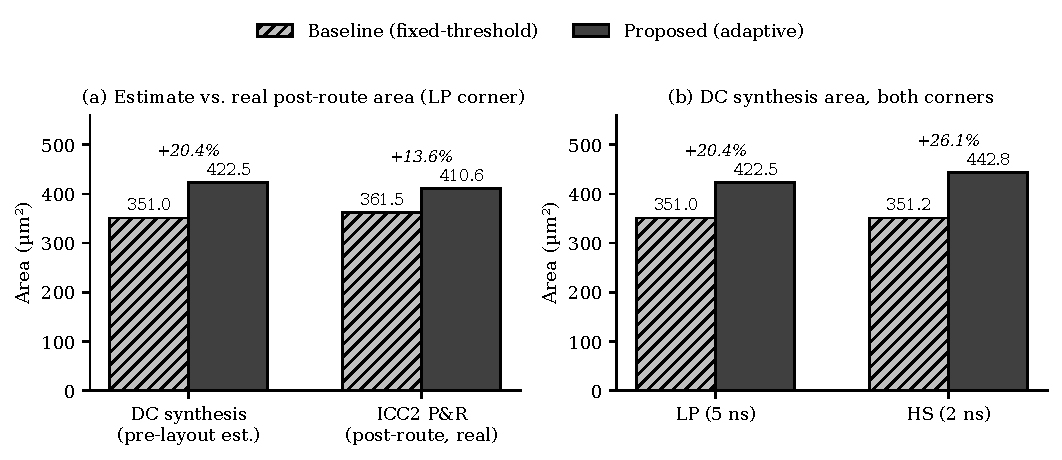
\includegraphics[width=\textwidth]{fig4_area_comparison.pdf}
\caption{(a) Pre-layout synthesis estimate vs.\ real post-route area at the low-power corner, and (b) DC synthesis area at both corners, baseline vs.\ proposed.}
\label{fig:area}
\end{figure*}

Tables~\ref{tab:area} \ref{tab:leakage} present the synthesis and post-route PPA results decomposed by metric category; Fig.~\ref{fig:area} visualizes the area trade-off.

%% ── Table III: Area ──────────────────────────────────────────────────────
\begin{table}[t]
\centering
\footnotesize
\caption{Cell Area Summary (DC Synthesis and Post-Route)}
\label{tab:area}
\setlength{\tabcolsep}{4pt}
\begin{tabular}{@{}l rrr@{}}
\toprule
Design point & Baseline ($\mu$m$^2$) & Proposed ($\mu$m$^2$) & Overhead \\
\midrule
DC synthesis, LP (5\,ns) & 350.98 & 422.51 & $+$20.4\% \\
DC synthesis, HS (2\,ns) & 351.25 & 442.76 & $+$26.1\% \\
Post-route (LP corner)   & 361.50 & 410.61 & $+$13.6\% \\
Post-route instances     & 1,014  & 1,118  & $+$10.3\% \\
\bottomrule
\end{tabular}
\end{table}

%% ── Table IV: Timing ─────────────────────────────────────────────────────
\begin{table}[t]
\centering
\small
\caption{Timing Closure Summary (DC Synthesis and Post-Route)}
\label{tab:timing}
\setlength{\tabcolsep}{5pt}
\begin{tabular}{l rr rr}
\toprule
 & \multicolumn{2}{c}{Baseline} & \multicolumn{2}{c}{Proposed} \\
\cmidrule(lr){2-3}\cmidrule(lr){4-5}
Corner & WNS (ns) & TNS (ns) & WNS (ns) & TNS (ns) \\
\midrule
DC, LP (5\,ns) & $+$2.44 & 0.00 & $+$2.51 & 0.00 \\
DC, HS (2\,ns) & $+$0.01 & 0.00 & $+$0.01 & 0.00 \\
Post-route, LP & $+$3.25 & 0.00 & $+$3.25 & 0.00 \\
\bottomrule
\multicolumn{5}{l}{\footnotesize WNS: worst negative slack (positive = timing met).} \\
\multicolumn{5}{l}{\footnotesize TNS: total negative slack (0.00 = no violations).} \\
\end{tabular}
\end{table}

%% ── Table V: Power ───────────────────────────────────────────────────────
\begin{table}[t]
\centering
\small
\caption{Power Summary -- DC Synthesis, LP Corner (5\,ns)}
\label{tab:power}
\setlength{\tabcolsep}{5pt}
\begin{tabular}{l rr r}
\toprule
Power metric & Baseline & Proposed & Overhead \\
\midrule
Cell internal power ($\mu$W)   & 7.09  & 13.54 & $+$91.0\% \\
Net switching power ($\mu$W)   & 4.71  & 5.64  & $+$19.7\% \\
Total dynamic power ($\mu$W)   & 11.80 & 19.18 & $+$62.5\% \\
Cell leakage power (nW)        & 627.2 & 991.3 & $+$58.0\% \\
\bottomrule
\multicolumn{4}{l}{\footnotesize Dynamic power at LP corner; leakage reflects always-on} \\
\multicolumn{4}{l}{\footnotesize controller cost, not runtime savings during sleep.} \\
\end{tabular}
\end{table}

%% ── Table VI: Post-route leakage ─────────────────────────────────────────
\begin{table}[t]
\centering
\small
\caption{Post-Route Static Leakage (LP Corner)}
\label{tab:leakage}
\setlength{\tabcolsep}{5pt}
\begin{tabular}{l rr r}
\toprule
Metric & Baseline & Proposed & Overhead \\
\midrule
Static leakage (pW)  & 115,164 & 138,428 & $+$20.2\% \\
Runtime saving, SPARSE (\%)  & 33.4 & 31.6 & $-$1.8\,pp \\
Runtime saving, MIXED (\%)   & 17.0 & 14.7 & $-$2.3\,pp \\
Runtime saving, BURST (\%)   & 8.8  & 0.7  & $-$8.1\,pp \\
\bottomrule
\multicolumn{4}{l}{\footnotesize Static leakage: full-power cost of controller logic.} \\
\multicolumn{4}{l}{\footnotesize Runtime saving: cycle-weighted leakage reduction during} \\
\multicolumn{4}{l}{\footnotesize actual workload execution (simulation measurement).} \\
\end{tabular}
\end{table}

The area results (Table~\ref{tab:area}) show a 13.6\% real post-route overhead, materially lower than the 20.4--26.1\% suggested by pre-layout DC estimation, reflecting tighter placement achieved by the Fusion Compiler router versus the wireload interconnect model. At the HS (2\,ns) corner, area overhead increases from 20.4\% to 26.1\% as DC inserts stronger drive-strength cells; both corners achieve positive worst-case slack (Table~\ref{tab:timing}), confirming timing feasibility across the explored frequency range. Post-route timing improves relative to DC estimates (WNS $+$3.25\,ns post-route vs.\ $+$2.51\,ns at DC synthesis) due to the router achieving shorter interconnect paths than the wireload model predicts.

The dynamic power overhead (Table~\ref{tab:power}) reflects the additional combinational logic in the always-on \textsf{PD\_TOP} domain: cell internal power increases by 91.0\% and switching power by 19.7\%, for a total dynamic overhead of 62.5\%. This is the at-speed cost of the controller logic itself. The post-route static leakage overhead of 20.2\% (Table~\ref{tab:leakage}) similarly measures the always-on controller cost at full supply; the realized runtime leakage savings -- 31.6\% under sparse, 14.7\% under mixed -- are the operational benefit, measured separately via the cycle-weighted simulation model. The cell placement across the 30$\times$30\,$\mu$m$^2$ floorplan is shown in Fig.~\ref{fig:placement}; the fully routed layout in Fig.~\ref{fig:layout}.

\begin{figure}[t]
\centering
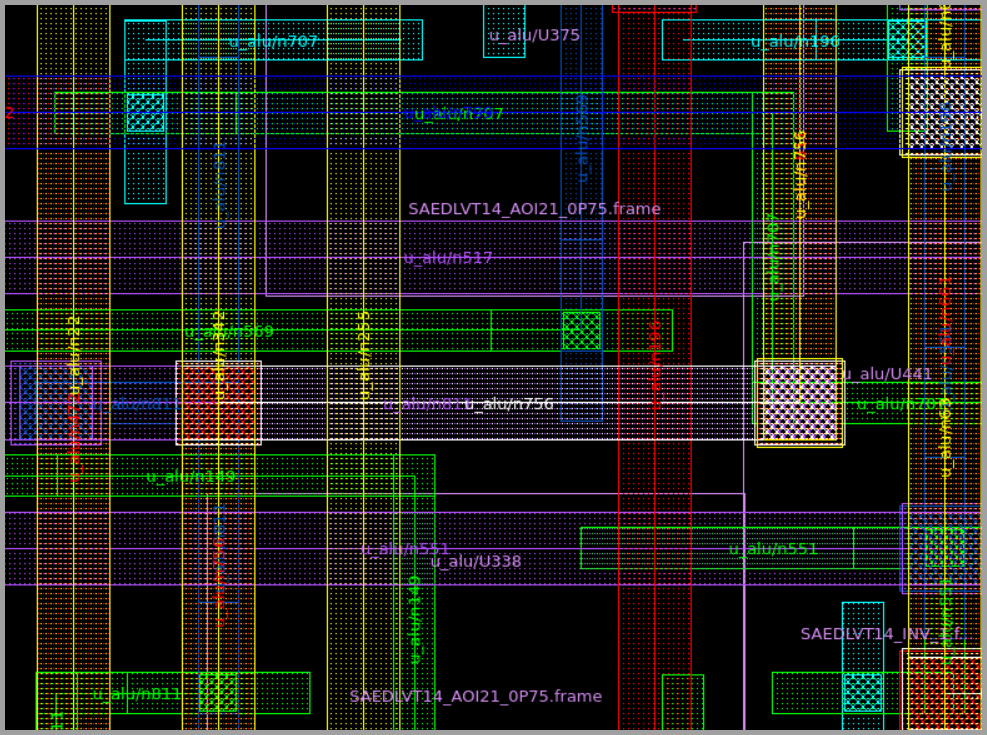
\includegraphics[width=\columnwidth]{fig10_layout_zoomed_nets.png}
\caption{Zoomed-in post-route view of the \texttt{u\_alu} region showing individual routed net labels (e.g., \texttt{u\_alu/n707}, \texttt{u\_alu/n517}) and standard-cell boundaries within a SAED14LVT \texttt{AOI21\_0P75} frame, illustrating the interconnect density resolved by the Fusion Compiler router.}
\label{fig:zoomed_nets}
\end{figure}

\begin{figure}[t]
\centering
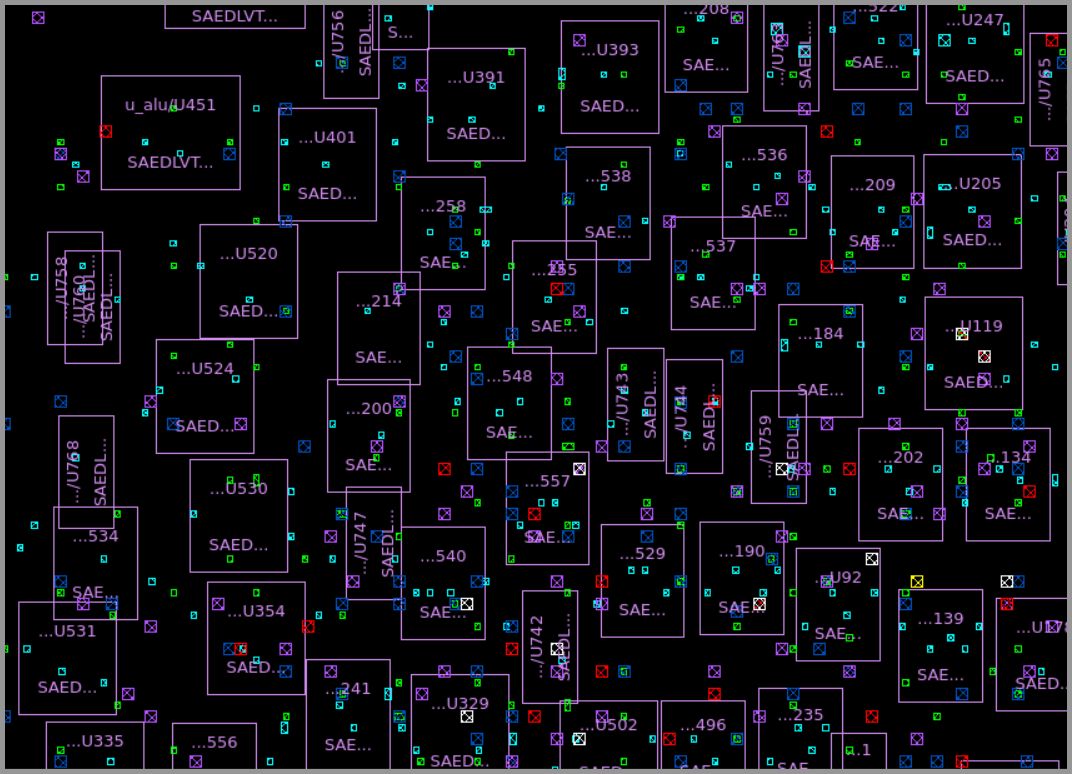
\includegraphics[width=\columnwidth]{fig11_layout_zoomed_cell_instances.png}
\caption{Zoomed-in cell-level view with instance labels (e.g., \texttt{U451}, \texttt{U401}, \texttt{U520}) overlaid on their corresponding SAED14LVT standard-cell footprints, illustrating instance-level placement density within the 30$\times$30\,$\mu$m$^2$ core.}
\label{fig:zoomed_cells}
\end{figure}

Figs.~\ref{fig:zoomed_nets} and \ref{fig:zoomed_cells} provide magnified detail of the post-route database underlying Fig.~\ref{fig:layout} and Fig.~\ref{fig:placement}: the former resolves individual net names and routing on a subset of the \texttt{u\_alu} datapath, and the latter isolates standard-cell instance boundaries and identifiers, confirming that the 1,118 placed instances are non-overlapping and legally aligned to the SAED 14\,nm LVT placement grid.

\section{Discussion}
\label{sec:discussion}

The central result of this work is the throughput preservation under bursty traffic shown in Section~\ref{sec:results}-A: a 3.1$\times$ throughput improvement over a representative fixed-threshold baseline, at zero mode transitions versus nineteen. This directly addresses the thrashing failure mode identified in Section~\ref{sec:related} and confirms the central novelty claim relative to \cite{agarwal2006}.

This benefit is not free. Real post-route synthesis shows a 13.6\% area overhead for the additional comparator and threshold-widening logic -- below the originally targeted 10\% ``lightweight'' threshold, but a substantial improvement over the 20--26\% suggested by pre-layout estimation alone. The appropriate framing for this result is a bounded, quantified trade-off rather than a cost-free improvement: comparator-based adaptive control achieves a meaningful behavioral improvement at a modest, real silicon cost, without resorting to the prediction-hardware overhead of learned approaches such as \cite{karthikeyan2025}. The 104 additional standard cells required for the adaptive predictor logic represent a minimal hardware investment compared to the ML inference hardware required by \cite{karthikeyan2025}.

Compared to prior work: versus \cite{agarwal2006}, this work adds the activity-rate second condition and eliminates thrashing under burst workloads. Versus \cite{karthikeyan2025}, this work achieves comparable qualitative adaptivity -- suppressing sleep during bursty periods, entering sleep during genuinely idle periods -- with no inference hardware, no learned models, and no per-cycle software classification. Versus \cite{chang2012}, this work's contribution is orthogonal: Chang et al.'s two-phase wake-up mechanism is adopted unchanged in both baseline and proposed designs as a shared constant.

\noindent\textit{Limitations:}
This work's energy comparisons use a derived metric -- transitions weighted by maximum wake-up latency -- rather than a first-principles joule measurement; a SPICE-level or annotated-switching-activity power simulation would strengthen this claim further. Post-route results are reported at a single LP corner; multi-corner PVT analysis was outside this project's scope. The synthetic workloads, while designed to specifically probe the threshold-crossing behavior under test, are not drawn from a real application trace. DRC verification was limited by the available PDK configuration on the server environment; the 7,376 spacing violations reported by the router reflect missing DRC deck rules rather than functional errors.

\section{Conclusion}
\label{sec:conclusion}

This work presented a comparator-based, dual-condition adaptive hysteresis controller for multi-level power gating, evaluated against a fair, structurally matched fixed-threshold baseline at both RTL-simulation and post-route physical-implementation levels. The proposed design eliminates sleep-state thrashing under bursty traffic, preserving throughput at 59.3\% versus 19.3\% for the fixed-threshold baseline -- a 3.1$\times$ improvement at zero mode transitions versus nineteen. Under genuinely sparse idle conditions, leakage savings converge to within 1.8 percentage points (31.6\% vs.\ 33.4\%), confirming the design does not sacrifice savings when idle conditions are unambiguous. The real post-route area overhead is 13.6\%, bounded and materially lower than the pre-layout synthesis estimate of 20--26\%. Timing closure is fully met at both LP (5\,ns) and HS (2\,ns) corners. The complete RTL-to-GDSII implementation was validated through Synopsys VCS functional simulation, DC Ultra synthesis, and Fusion Compiler place-and-route, with 0 open nets and a post-route worst-case slack of 3.25\,ns.

Future work includes extending the activity-rate gate to additional functional-block types beyond the ALU, multi-corner PVT physical verification, SPICE-level energy measurement to replace the derived transition-cost proxy metric, and validation against real application traces rather than synthetic workloads.

\subsection*{Code Availability}
The RTL, testbench, UPF power intent, and synthesis/place-and-route scripts used in this work are available at \url{https://github.com/JHT127/hysteresis-adaptive-power-gating}.


\bibliographystyle{IEEEtran}
\bibliography{references}

\end{document}
